% !TeX root = chapter4_2d_new.tex
% !TeX root = thesis.tex
\ifdefined\UtilIncluded
  \renewcommand{\startchapter}[1]{}
  \renewcommand{\stopchapter}{}
  \renewcommand{\undefinedlabel}[2]{}
\else

\newcommand{\startchapter}[1]{\begin{document}\setcounter{chapter}{#1}\addtocounter{chapter}{-1}}
\newcommand{\stopchapter}{\printbibliography[title=Bibliography,heading=bibintoc]\end{document}}


\documentclass{book}
\usepackage[utf8]{inputenc}


\usepackage{geometry}
\geometry{
  papersize={170mm,240mm},
}

\usepackage{amsfonts,amsmath, amsthm, amssymb, mathtools}
\usepackage{xspace}
\usepackage[hidelinks,bookmarks,pdfusetitle]{hyperref}
\usepackage{listings}
\usepackage[pdftex]{graphicx}
\usepackage{bm}
\usepackage[english]{babel}
\usepackage{caption}
\usepackage{subcaption}
\usepackage[usenames,dvipsnames]{xcolor}
\usepackage{physics}
\usepackage{multicol}
\usepackage{xstring}
\usepackage{pythonhighlight}
\usepackage{parskip}
\usepackage{thmtools}
\usepackage{relsize}
\usepackage{bookmark}
\usepackage{lmodern}
\usepackage{ifthen}
\usepackage{biblatex}
\usepackage{microtype}
\usepackage{csquotes}
\usepackage{numprint}
\usepackage{mleftright}
\npthousandsep{{\ifmmode\mskip2mu\else\hskip0.2em\fi}}
\npdecimalsign{.}

\addbibresource{references.bib}

\newtheorem{theorem}{Theorem}[chapter]
\newtheorem{lemma}[theorem]{Lemma}
\newtheorem{corollary}[theorem]{Corollary}
\newtheorem{definition}[theorem]{Definition}

\DeclareRobustCommand{\oneD}{{1{\relsize{-1}D}}\xspace}
\DeclareRobustCommand{\twoD}{{2{\relsize{-1}D}}\xspace}
\DeclareRobustCommand{\threeD}{{3{\relsize{-1}D}}\xspace}
\DeclareRobustCommand{\cpp}{{{C\nolinebreak[4]\hspace{-.05em}\raisebox{.4ex}{\relsize{-3}\textbf{++}}}\xspace}}
\pdfstringdefDisableCommands{%
  \def\cpp{C++}%
  \def\oneD{1D}%
  \def\twoD{2D}%
  \def\threeD{3D}%
}

\newcommand{\longchapter}[2][]{%
  \chapter[#2]{#2}%
  \ifthenelse{\equal{#1}{}}{}{\chaptermark{#1}}}

\newcommand{\NN}{\mathbb{N}}
\newcommand{\ZZ}{\mathbb{Z}}
\newcommand{\QQ}{\mathbb{Q}}
\newcommand{\QQbar}{\overline{\mathbb{Q}}}
\newcommand{\RR}{\mathbb{R}}
\newcommand{\CC}{\mathbb{C}}

\newcommand{\Eigen}{\texttt{Eigen}}

\newcommand{\sage}{\texttt{sage}\xspace}

\newcommand{\hamiltonian}{\mathcal{H}}

\newcommand{\transposesign}{\intercal}
\newcommand{\transpose}[1]{{#1}^\transposesign}
\newcommand{\adjointsign}{\text{H}}
\newcommand{\adjoint}[1]{{#1}^\adjointsign}

\newcommand{\xmin}{{x_{\text{min}}}}
\newcommand{\xmax}{{x_{\text{max}}}}
\newcommand{\ymin}{{y_{\text{min}}}}
\newcommand{\ymax}{{y_{\text{max}}}}

\newcommand{\Cbottom}{\vb{C}_\text{bottom}}
\newcommand{\Ctop}{\vb{C}_\text{top}}
\newcommand{\ubottom}{\vb{u}_\text{bottom}}
\newcommand{\utop}{\vb{u}_\text{top}}

\DeclareMathOperator{\diag}{diag}
\DeclareMathOperator{\tridiag}{tridiag}
\DeclareMathOperator{\eigs}{eigs}
\DeclareMathOperator*{\argmin}{arg\,min}
\DeclareMathOperator{\Ai}{Ai}
\DeclareMathOperator{\Bi}{Bi}
\DeclareMathOperator{\OO}{\mathcal{O}}

% https://tex.stackexchange.com/a/18192/163747
\makeatletter
\newcommand{\undefinedlabel}[2]{%
  \protected@write \@auxout {}{\string \newlabel {#1}{{#2}{\thepage}{#2}{#1}{}} }%
  \hypertarget{#1}{}
}
\makeatother

\fi
\gdef\UtilIncluded{}


\startchapter{4}
\undefinedlabel{cha:c2}{2}
\undefinedlabel{cha:c3}{3}

\longchapter[New methods]{New methods for the \twoD time-independent Schrödinger equation}\label{cha:c4}

In chapter \ref{cha:c2} we have studied the constant perturbation methods. We have seen a brief history about these CP-methods, as well as, a thorough overview about how these methods can be implemented. The numerical examples illustrated the benefits and demonstrated the accuracy of the studied techniques.

Chapter \ref{cha:c3} was dedicated to the treatment of a recent method to solve the time-independent two-dimensional Schrödinger equation. This method aims to use the strengths of the constant perturbation methods for higher dimensional problems. This new method is promising, and we developed many improvements upon the original idea.

One of the unique powers of the CP-methods was their ability to not only compute low eigenvalues accurately, but even increase accuracy for higher eigenvalues. This is one of the few, if not the only, method which has this very desirable property for Sturm-Liouville problems. For two dimensions, this property did not translate cleanly. The method described in chapter \ref{cha:c3} tries to capture this by considering solutions of a one-dimensional Schrödinger problem in the $x$-direction. And a method for a coupled system of Schrödinger equations has been used in the $y$-direction. In theory this method is capable of computing any eigenvalue. In practice, this is not the case. Along the $x$-direction an eigenfunction is represented as a linear combination of basis functions. This basis is well-chosen, such that only a few number of functions are able to capture the true eigenfunctions sufficiently. Yet, as computers are finite, this basis has to be this as well. As eigenfunctions corresponding to higher eigenvalues will become more and more oscillatory, the chosen finite basis will no longer be able to express all necessary details.

That the basis is finite, thus, limits the accuracy for higher eigenvalues. Which negates one of the strongest benefits of the employed CP-methods. As such, we believe that the utopian method for the more-dimensional time-independent Schrödinger equation, is one which does not decrease in accuracy, as the higher eigenvalues are requested. Just like the CP-methods are for the one-dimensional case. Developing such a method will, most likely, require new and very complicated formulae.

For clarity, we did not develop such a perfect method. But in the last few years I've played with the idea... In section \ref{c4:sec_utopy} we will present some ideas for such a method. Some of which, someone, somewhere, may find inspirational.

More realistically, during our research into the method of Ixaru, we have found other research, also focussing upon the time-independent Schrödinger problem. These ideas and methods have inspired us to develop our own technique. The new methods we propose try to fix or mitigate some issues present in the other methods.

    {\color{red} To do: list other methods}

\section{Inspiration}

After careful implementation and thorough testing of Ixaru's method from chapter \ref{cha:c3}, I could browse through the literature with renewed appreciation for the Schrödinger problem. When researching that method, many obstacles and challenges arose. It was an interesting task to balance computation time, symbolic formulas and numerical accuracy. So with this in mind, I came across \cite{wang_new_2009} by Wang and Shao.

In this article they proposed a new kind of discretization scheme for solving two-dimensional time-independent Schrödinger equations. Before studying the details of the method, I like to review the numerical results. They tested their algorithm on two potential functions. Firstly, the harmonic oscillator: Schrödinger equations with this potential function are not extremely difficult, but it captures some of the challenges that numerical algorithms may face, while still having symbolic solutions for the eigenvalues. Secondly, they provided results for the Hénon-Heiles potential. Here, the exact solutions are not known, but reliable approximations exist. For both potentials their results were quite impressive. The reached high accuracy, for a significant number of eigenvalues, without using excessive computation time.

But the thing that strikes me most about \cite{wang_new_2009} is the simplicity of their method. They constructed formulas for a direct discrete approximation on a grid. Finding these kinds of results within the literature is disheartening and inspirational at the same time. At first glance they were able to reach higher accuracy with a simpler method than Ixaru's work \cite{ixaru_new_2010} and our improvements \cite{baeyens_improvements_2022} to it. Before throwing away all our work, and declaring \cite{wang_new_2009} to be superior, let us analyze it ourselves.

\subsection{A finite difference scheme}

In \cite{wang_new_2009} they discretize space with an equidistant $n_x \times n_y$ grid. With this, they approximate the second partial derivative of a function $\psi(x, y)$ with, what they call, a new scheme:
$$
    {\pdv[2]{}{x}}\psi(x, y) = -\frac{1}{h^2}\sum_{i=-N_q}{N_q} c_i \psi(x + ih, y)\text{.}
$$
In this expression $h$ is the $x$-step of the equidistant grid. An analogous formula for the second partial derivative of $\psi(x, y)$ with respect to $y$ is proposed, with $y$-step $\eta$:
$$
    {\pdv[2]{}{y}}\psi(x, y) = -\frac{1}{\eta^2}\sum_{i=-N_q}{N_q} c_i \psi(x, y + i\eta)\text{.}
$$

To determine the value of $c_i$, the authors propose to use the Taylor series expansion of
$$
    \left({\pdv[2]{}{x}} + {\pdv[2]{}{y}}\right)\psi(x, y) = -\frac{1}{h^2} \sum_{i=-N_q}^{N_q} c_i \left(\psi(x+ih, y) + \left(\frac{h}{\eta}\right)^2\psi(x, y+i\eta)\right)\text{.}
$$
In \cite{wang_new_2009} the coefficients $c_i$ for $N_q = 3, 4, 5, 6$ are provided. If we restrict the Schrödinger equation to the domain $[-R_x, R_x] \times [-R_y, R_y]$ the authors propose to assume all eigenfunctions will be zero outside this region. This way, their formulae, for a fixed $N_q$ can still be used, even for grid points close to the edge of the domain.

Using these formulae the problem now approximates to a simple, albeit very large, square matrix eigenvalue problem.
\begin{equation}\label{equ:c4_fd_sparse_matrix}
    \left(-\vb{D}_{n_x} \otimes \vb{I}_{n_y} - \vb{I}_{n_x} \otimes \vb{D}_{n_y} +  \diag\begin{pmatrix}V(x_1, y_1) \\ V(x_1, y_2) \\ \vdots \end{pmatrix} \right)\vb{u} = \lambda \vb{u}
\end{equation}
Here, $\vb{D}_{n_x}$ is the symmetric Toeplitz\footnote{A matrix is called Toeplitz if each diagonal only contains a constant value. In other words, a matrix $\vb{A}$ is Toeplitz if it can be written as follows. $\vb{A}$ is a symmetric Toeplitz matrix if $a_{-i} = a_i$. $$\begin{pmatrix} a_0 & a_1 & a_2 & \dots \\ a_{-1} & a_0 & a_1 & \ddots \\ \vdots & \ddots & \ddots & \ddots \end{pmatrix}$$} $n_x \times n_x$ matrix with the first row $\begin{pmatrix} c_0 & c_1 & \dots & c_{N_x} & 0 & \dots \end{pmatrix}$. Analogous for $\vb{D}_{n_y}$. The $n\times n$ identity matrix is denoted as $\vb{I}_n$. The operation $\cdot \otimes \cdot$ is the Kronecker product\footnote{The Kronecker product of the $m\times m$ matrix $\vb{A}$ and the $n\times n$ matrix $\vb{B}$ is the following $(m+n)\times (m+n)$ block matrix: $$ \vb{A} \otimes \vb{B} = \begin{pmatrix} A_{1,1} \vb{B} & A_{1,2} \vb{B} & \dots \\ A_{2,1} \vb{B} & A_{2,2} \vb{B} & \\ \vdots & & \ddots \end{pmatrix} $$}. And finally, the vector of unknowns $\vb{u}$ is the approximation of $\psi$ in each of the grid points: $\vb{u} \approx \transpose{\begin{pmatrix} \psi(x_1, y_1) & \psi(x_1, y_2) & \dots \end{pmatrix}}$. The matrix on the left-hand side of \eqref{equ:c4_fd_sparse_matrix} can be directly computed. It is valuable to note that most of the entries of this matrix will be zero, so considering it as a sparse matrix is preferred. Many classical, well tested,  solvers exist for sparse eigenvalue problems. The authors of \cite{wang_new_2009} have used algorithms provided by Mathematica.

Before reviewing, and recalculating their numerical results, I want to take the time to thoroughly analyze their formulae. Using an equidistant grid and coefficients which optimize for the Taylor series of the function in question, is oddly reminiscent of finite difference approximations. To confirm this similarity we have calculated the central finite difference approximations of the second order derivative.

The following table contains the first few central symmetric finite differences.
\begin{center}
    \begin{tabular}{r|ccccccccccc}
Order & $c_0$ & $c_{-1}=c_{1}$ & $c_{-2}=c_{2}$ & $c_{-3}=c_{3}$ & $c_{-4}=c_{4}$ & $c_{-5}=c_{5}$\\[2pt]\hline
2 & $-2$ & $1$ & & & &\\[4pt]
4 & $- \frac{5}{2}$ & $\frac{4}{3}$ & $- \frac{1}{12}$ & & &\\[4pt]
6 & $- \frac{49}{18}$ & $\frac{3}{2}$ & $- \frac{3}{20}$ & $\frac{1}{90}$ & &\\[4pt]
8 & $- \frac{205}{72}$ & $\frac{8}{5}$ & $- \frac{1}{5}$ & $\frac{8}{315}$ & $- \frac{1}{560}$ &\\[4pt]
10 & $- \frac{5269}{1800}$ & $\frac{5}{3}$ & $- \frac{5}{21}$ & $\frac{5}{126}$ & $- \frac{5}{1008}$ & $\frac{1}{3150}$
\end{tabular}

\end{center}

As one sees, these give exactly the same coefficients as in \cite{wang_new_2009}. It is quite disingenuous to call this a \emph{new} scheme. The study of finite difference can be traced back to, among others, Newton. One of the first English books was by Boole \cite{boole_calculus_1860} in 1860, with many more textbooks to follow \cite{thomson_calculus_1933,jordan_calculus_1965}. Even the symbolic construction of high order approximations has already been studied and tabulated as early as 1967 \cite{ballester_construction_1967,keller_symbolic_1978,fornberg_generation_1988}.


Besides this remark, \cite{wang_new_2009} is very valuable as an application of very high orders of these well-known formulae to the two-dimensional time-independent Schrödinger equation. Their numerical results are still valid and nonetheless impressive.

\subsubsection{Numerical experiments with high order finite difference approximations}

\begin{figure}
    \begin{center}
        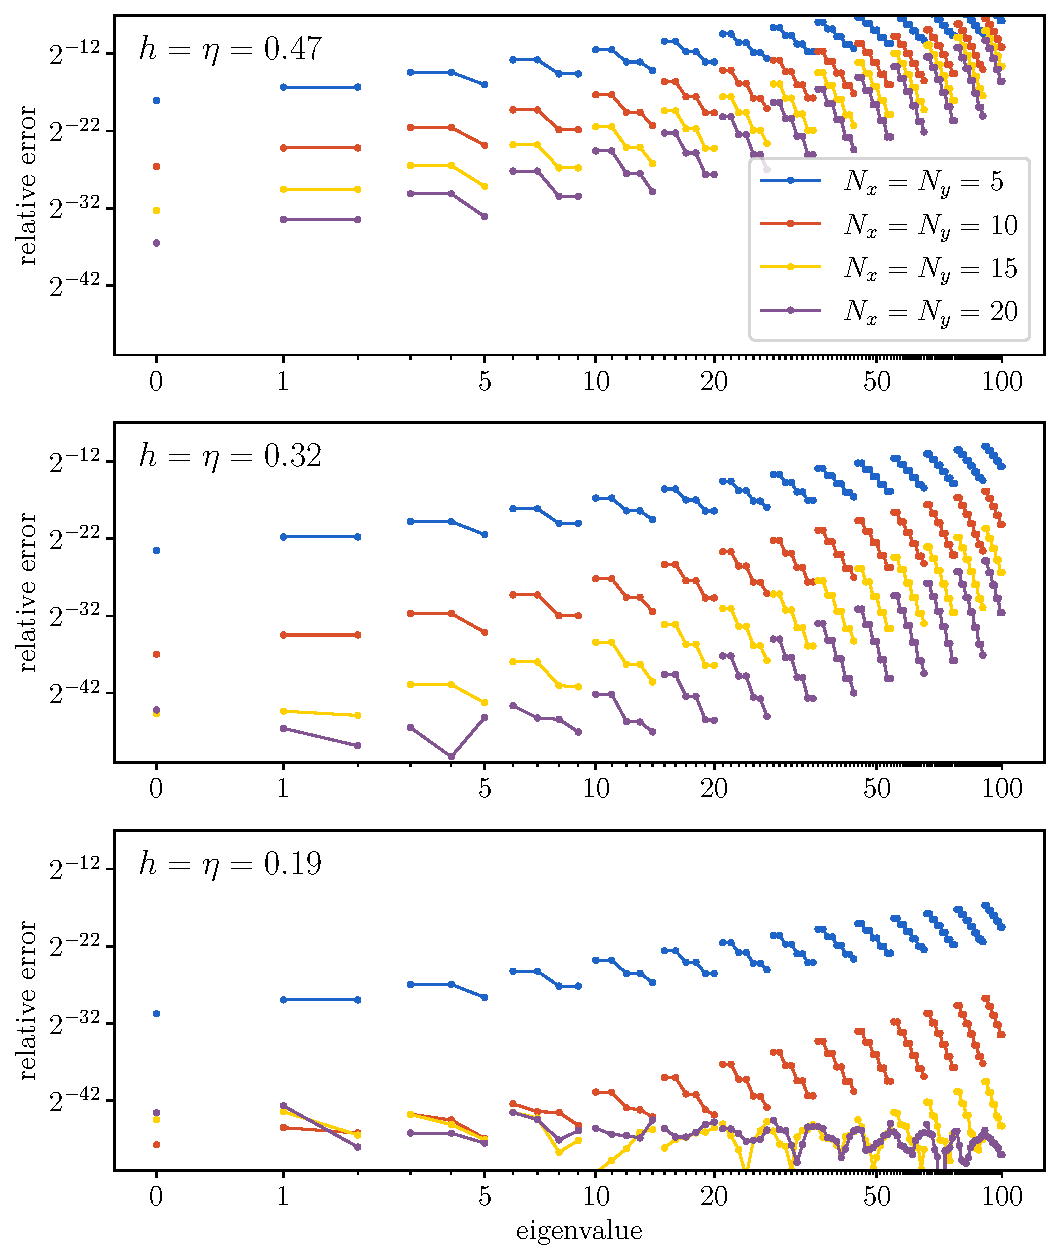
\includegraphics[width=\textwidth]{img/chapter4/fd_harmonic.pdf}
    \end{center}
    \caption{These graphs display the relative error of each of the first $100$ eigenvalues of the harmonic oscillator \eqref{equ:c4_fd_harmonic}, computed for different values of $h = \eta$ and $N_x = N_y$. Repeated eigenvalue are connected.}
    \label{fig:c4_fd_harmonic}
\end{figure}

As a first example we will replicate the results of \cite{wang_new_2009} for the harmonic oscillator:
\begin{equation}\label{equ:c4_fd_harmonic}
    -\nabla^2 \psi(x, y) + \left(x^2 + y^2\right) \psi(x, y) = E \psi(x, y)
\end{equation}
on the domain $[\numprint{-9.5}, \numprint{9.5}] \times [\numprint{-9.5}, \numprint{9.5}]$ with homogeneous Dirichlet boundary conditions. Notice that in \cite{wang_new_2009} the authors have chosen to scale the potential and eigenvalue by an extra factor of two. Here we did not do this, as such are computed eigenvalues will be twice as large. But, the relative error still can be compared.

In figure \ref{fig:c4_fd_harmonic} the relative errors for the first $100$ eigenvalues are plotted. This is done for $h = \eta \in \left\{\frac{19}{40}, \frac{19}{60}, \frac{19}{100}\right\}$ and $N_x = N_y \in \left\{ 5, 10, 20, 25 \right\}$. In these graphs a few things can be noted. Unsurprisingly, when $N_x = N_y$ is increased, the results become more accurate. And also, when $h = \eta$ is decreased, that is to say more grid points are used, the results also become more accurate. As is the case with most algorithms for approximating Schrödinger equations, when larger eigenvalues are computed, the accuracy decreases. The corresponding eigenfunctions become more and more oscillatory, and are thus more difficult to approximate accurately.

But most impressively, all these graphs were computed within a minute on a simple laptop. More detailed runtime analysis can be found in section \ref{sec:c4_nm_vs_fd}. Furthermore, the obtained results are also impressive. In the most accurate case $h= \eta = \frac{19}{100}$ and $N_x = N_y = 20$, the first $100$ eigenvalues are found with $45$ bits of precision, which is close to the ideal machine precision of $53$ bits.

To get a deeper understanding of this finite difference method it may be beneficial to study the asymptotic behavior of the error. In theory the finite difference approximation error can be used as a jumping point. Assume $N = N_x = N_y$, then the finite difference approximation of the second derivative of a function $f : \RR \to \RR$ is of the form:
$$
    f''(x) = \frac{1}{h^2}\sum_{i=-N}^{N} c_{i} f(x + i h) + \OO\mleft(h^{2N}\mright)\text{.}
$$

Going further with a theoretical analysis becomes unnecessarily difficult. We will estimate the order by using the numerical results for the first $100$ eigenvalues of the harmonic oscillator, calculated for the values of $h = \eta = \frac{1}{n}$ for $n \in \left\{20, 30, 40, 50, 60, 70, 80, 90, 100\right\}$. These $9$ different sets of parameters yield for each of the $100$ eigenvalues (with index $k \in \{1, 2, \dots, 100\}$) a data point. Next, through all these points we find the best fitting curve which follows the formula $c_1 h^{c_2} k^{c_3}$. In this case we define the best fitting curve to be such that for the error $\epsilon_k^{(h)}$ (for each eigenvalue $k$ calculated with a step size of $h = \eta$), the following is minimized:
$$
    \sum_{k, h}\left|\log|\epsilon_{k}^{(h)}| - \log\mleft(c_1 h^{c_2} k^{c_3}\mright)\right|^2 \text{.}
$$

These best fits are summarized in the following table.
\begin{center}
    \begin{tabular}{r|cccc}
$N_x = N_y$ & $5$ & $10$ & $15$ & $20$ \\\hline\rule{0pt}{2.6ex}
Error & $\OO\mleft(h^{\numprint{3.90}}k^{\numprint{2.96}}\mright)$ & $\OO\mleft(h^{\numprint{5.78}}k^{\numprint{2.92}}\mright)$ & $\OO\mleft(h^{\numprint{6.61}}k^{\numprint{2.86}}\mright)$ & $\OO\mleft(h^{\numprint{7.07}}k^{\numprint{2.83}}\mright)$
\end{tabular}

\end{center}

It is important to note that these values or estimates, and quite sensitive to the used values of $n$ and $k$. But, some trends are visible. We first note that increasing $N$ indeed increases the order in $h$ as well, maybe not as much as theoretical assumed $\OO\mleft(h^{2N}\mright)$, but nonetheless significantly. Another visible behavior is that a more accurate (higher order in $h$) method also has a larger exponent with respect to $k$. This means that higher eigenvalues are asymptotically less accurate. This property can also be seen in the graphs of figure \ref{fig:c4_fd_harmonic}, a virtual line through the points corresponding to $N = 5$ is less steep than a line through the points of $N = 10$. For one-dimensional problems the order in function of $k$ has already been well studied. In \cite{paine_correction_1981} expressions are constructed which provide a correction to the numeric approximation with finite difference schemes for Sturm-Liouville problems. These correction formulae bring the order in k down from $\OO(k^4h^2)$ to $\OO(k h^2)$. For multidimensional Schrödinger equations no such corrections are available, let alone for the extremely high order schemes considered here.

Besides the harmonic oscillator it is also instructive to consider the problem with a zero potential function on the domain $[0, \pi] \times [0, \pi]$ and homogeneous Dirichlet boundary conditions:
\begin{equation}\label{equ:c4_fd_zero}
    -\nabla^2 \psi(x, y) = E \psi(x, y) \text{.}
\end{equation}

\begin{figure}
    \begin{center}
        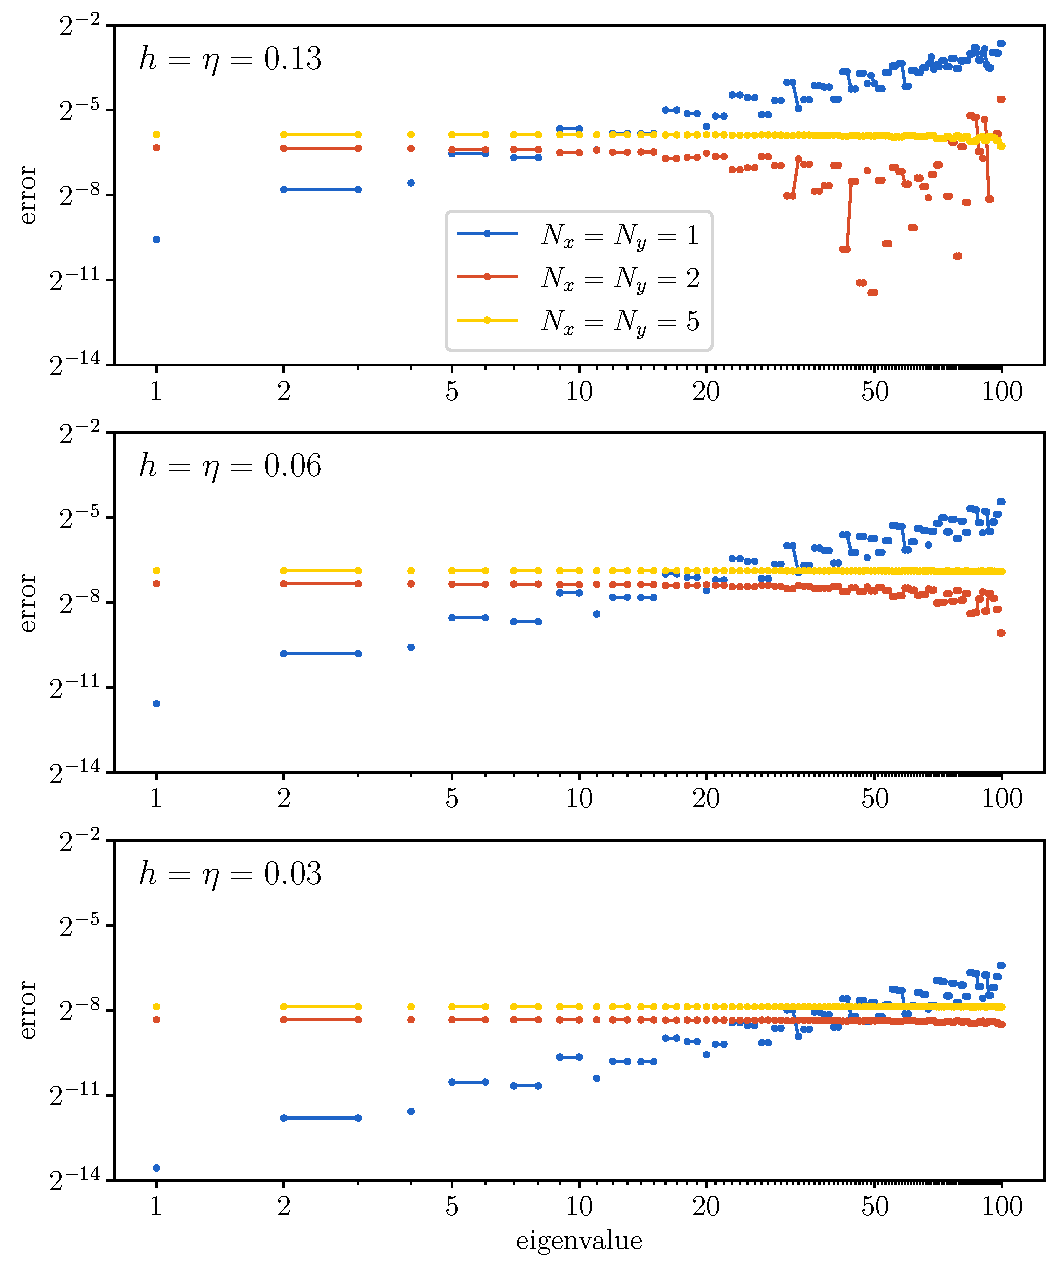
\includegraphics[width=\textwidth]{img/chapter4/fd_zero.pdf}
    \end{center}
    \caption{These graphs display the relative error of each of the first $100$ eigenvalues of the zero potential \eqref{equ:c4_fd_zero}, computed for different values of $h = \eta$ and $N_x = N_y$. Repeated eigenvalue are connected.}
    \label{fig:c4_fd_zero}
\end{figure}

By separation of variables, the exact solutions of this equation can be found: $\psi_{i, j}(x, y) = \sin(i x)\sin(j y)$ with eigenvalue $\lambda_{i,j} = i^2 + j^2$ for all $i, j \in \NN_{>0}$. The first few of these eigenvalues are listed.
\begin{align*}
\lambda_{1,1} &= 2 & \lambda_{3,3} &= 18 & \lambda_{3,5} = \lambda_{5,3} &= 34\\
\lambda_{1,2} = \lambda_{2,1} &= 5 & \lambda_{2,4} = \lambda_{4,2} &= 20 & \lambda_{1,6} = \lambda_{6,1} &= 37\\
\lambda_{2,2} &= 8 & \lambda_{3,4} = \lambda_{4,3} &= 25 & \lambda_{2,6} = \lambda_{6,2} &= 40\\
\lambda_{1,3} = \lambda_{3,1} &= 10 & \lambda_{1,5} = \lambda_{5,1} &= 26 & \lambda_{4,5} = \lambda_{5,4} &= 41\\
\lambda_{2,3} = \lambda_{3,2} &= 13 & \lambda_{2,5} = \lambda_{5,2} &= 29 & \lambda_{3,6} = \lambda_{6,3} &= 45\\
\lambda_{1,4} = \lambda_{4,1} &= 17 & \lambda_{4,4} &= 32 & \lambda_{1,7} = \lambda_{5,5} = \lambda_{7,1} &= 50
\end{align*}%

In a certain way, these eigenvalues are more interesting than those from the harmonic oscillator, as their multiplicities are less predictable.

In figure \ref{fig:c4_fd_zero} the error on each of the first $100$ eigenvalues is displayed for different values of $h = \eta$ and $N_x = N_y$. When comparing this figure to the results of the harmonic oscillator \ref{fig:c4_fd_harmonic}, some striking differences can be seen. Maybe most surprisingly, increasing the order does not give more accurate results! For low eigenvalues the method with $N_x=N_y=1$ is most accurate, this is simply the second order central finite difference formula. When using higher order methods the error does not get any better than $2^{-8}\approx \numprint{0.00391}$. Which is not at all as accurate as the results for the harmonic oscillator, where the error for $N_x=N_y = 5$ lies between $2^{-32} \approx \numprint{2.3e-10}$ and at most $2^{-16} \approx \numprint{1.5e-05}$. This is quite a disconcerting behavior for a numerical method to have.

These results bring to light one of the biggest drawbacks of the method from \cite{wang_new_2009}. This method only works if it is assumed that the eigenfunctions always are zero outside the domain. For the harmonic oscillator, this is the case, as $V(x, y) \to +\infty$ if $\|x, y\| \to +\infty$. For the zero potential function this is definitely not the case, the eigenfunctions are periodic. One could argue that, in theory, an eigenfunction may be anything outside the domain $\Omega$. So in particular, we could define them to be zero there. But, most numerical methods, and this method in particular, assume that solutions are sufficiently continuous. To cleanly define the problem, at least $C_0^2(\Omega)$ is needed, and when using $N^\text{th}$ order central finite difference schemes are used $C_0^{N}(\Omega)$ is implicitly assumed. And this assumption fails if we define the function to be zero outside $\Omega$.

To combat this issue, on the boundary of the domain asymmetric schemes could be used, the authors of \cite{wang_new_2009} did not do this. As an example, we have tabulated all relevant six point formulae.
\begin{center}
    \begin{tabular}{ccc|c|ccccc|r}
$c_{-3}$ & $c_{-2}$ & $c_{-1}$ & $c_{0}$ & $c_{1}$ & $c_{2}$ & $c_{3}$ & $c_{4}$ & $c_{5}$ & error \\\hline
\rule{0pt}{3ex} $\frac{1}{90}$ & $- \frac{3}{20}$ & $\frac{3}{2}$ & $- \frac{49}{18}$ & $\frac{3}{2}$ & $- \frac{3}{20}$ & $\frac{1}{90}$ &  &  & $\OO\mleft(h^{6}\mright)$ \\
\rule{0pt}{3ex}  & $- \frac{13}{180}$ & $\frac{19}{15}$ & $- \frac{7}{3}$ & $\frac{10}{9}$ & $\frac{1}{12}$ & $- \frac{1}{15}$ & $\frac{1}{90}$ &  & $\OO\mleft(h^{5}\mright)$ \\
\rule{0pt}{3ex}  &  & $\frac{137}{180}$ & $- \frac{49}{60}$ & $- \frac{17}{12}$ & $\frac{47}{18}$ & $- \frac{19}{12}$ & $\frac{31}{60}$ & $- \frac{13}{180}$ & $\OO\mleft(h^{5}\mright)$ \\
\end{tabular}

\end{center}
There are two difficulties when using these formulae. Firstly, to reach the required order, one point more should be used. And secondly, when using asymmetric formulae the matrix from \eqref{equ:c4_fd_sparse_matrix} looses its symmetry as well. In principle this should not matter. But, in practice, many sparse matrix eigenvalue solvers are much more efficient when working with a real symmetric matrix.




    {\color{red}To do: Hénon-Heiles}


\subsubsection{Computational cost of the method}

Finite differences are employed in many real-world applications, as they are easy to implement, yet are able to reach high accuracies. In practice, however, it is rare to see these very high orders used. In this setting these high orders seem to be very well applicable.

Yet, these finite difference methods are not without issues. One of the most prominent drawbacks is the expensive computations involved. To get accurate results high orders, combined with large grids, have to be used. This results in huge, sparse, matrices. And only thanks to their sparsity are algorithms able to compute the eigenvalues. Now, for higher order schemes, the matrices become less sparse, and as such more expensive to work with.

Alternatively, a method which is able to reduce the size of the matrices involved without losing accuracy may be preferable.

    {\color{red}To do

        \begin{enumerate}
            \item Do not assume zero outside domain
            \item High orders loose sparsity
        \end{enumerate}

    }

\subsection{A semi-discrete method}\label{sec:c4_semi_discrete}

\section{A woven interpolation method}

In contrast to the previous methods, we propose a technique which is not necessarily restricted to cases where the domain is only a rectangle. So consider a finite domain $\Omega \subseteq \RR$ on which we are searching eigenvalues $E \in \RR$ and eigenfunctions $\psi: \Omega \to \RR$ such that for a given potential $V : \Omega \to \RR$ the following holds
\begin{equation}\label{equ:c4_schrodinger_equation_new_method}
    -\nabla^2 \psi + V(x, y) \psi = E \psi\text{.}
\end{equation}
Still, we impose homogeneous Dirichlet boundary conditions, thus, $\psi(x, y) = 0$ for $(x, y) \in \Omega$.

The main idea underlying this method is that we want to represent the eigenfunctions $\psi$ efficiently. A fully discretized method may represent eigenfunctions as it's values on certain grid points. Our first attempt to develop a more continuous approximation of the eigenfunction used ideas from chapter \ref{cha:c3} and led to the creation of section \ref{sec:c4_semi_discrete}. Here we have chosen to approximate the eigenfunction as a linear combination of well-chosen basis functions on parallel lines throughout the domain. This led to a continuous approximation along one direction and a discrete approximation along the other direction of the domain.

\begin{figure}
    \begin{center}
        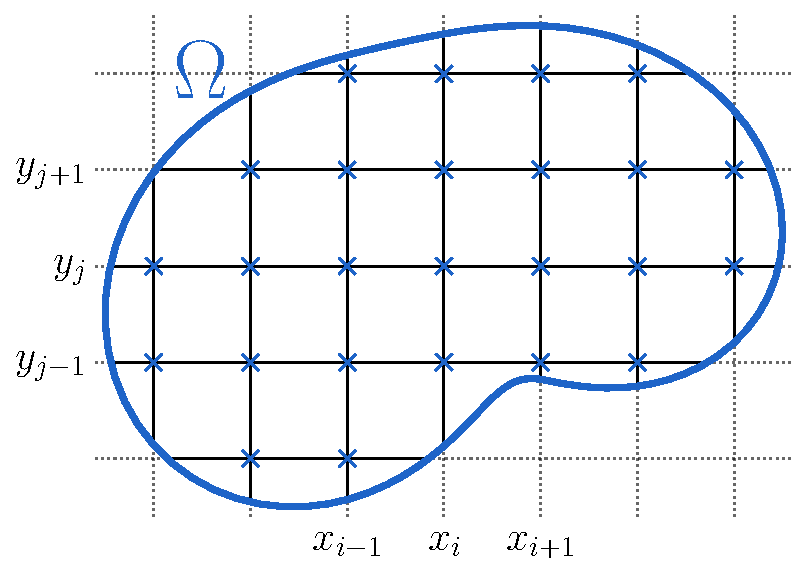
\includegraphics[width=.8\linewidth]{img/chapter4/the_method_grid.pdf}
        \caption{\label{fig:woven_method_grid} The grid}
    \end{center}
\end{figure}

In this new method we will bring this continuous approximation to both directions of the domain. For this, we place a grid over the domain $\Omega$, as can be seen in figure \ref{fig:woven_method_grid}. This grid need not be equidistant or square. When developing this new method we strived to allow for maximal flexibility, by avoiding as many restrictions on $\Omega$ as possible. This has as consequence that, because $\Omega$ does not have to be a rectangle, the number of intersections per grid line is not necessarily constant. Upon formulating and implementing this new method, this varying number of intersections is one example of some difficulties that arise by explicitly allowing more flexibility.

After placing the grid on $\Omega$, the next step is to approximate the unknown eigenfunction $\psi$ as a linear combination of basis functions on each of the grid lines. On the vertical line $x = x_i$, we denote these basis functions as $\beta_k^{(x_i)}(y)$, for each value of $k$. This yields the expression
$$
    \psi(x_i, y) = \sum_{k=0}^\infty c_k^{(x_i)} \beta_k^{(x_i)}(y) \text{.}
$$
For horizontal lines $y = y_j$, the basis functions $\beta_k^{(y_j)}(x)$ yield a similar expression
$$
    \psi(x, y_j) = \sum_{k=0}^\infty c_k^{(y_j)} \beta_k^{(y_j)}(x) \text{.}
$$

To ensure $\psi(x, y)$ is uniquely defined in each point in $\Omega$ we have to require that in each intersection point $(x_i, y_j)$, $\psi(x_i, y_j)$ has only one solution:
\begin{equation}\label{equ:c4_new_method_pre_matrix_equality}
    \psi(x_i, y_j) = \sum_{k=0}^\infty c_k^{(x_i)} \beta_k^{(x_i)}(y_j) = \sum_{k=0}^\infty c_k^{(y_j)} \beta_k^{(y_j)}(x_i)\text{.}
\end{equation}

Before deciding on which basis functions we should use, let us consider the Schrödinger equation \eqref{equ:c4_schrodinger_equation_new_method} on each intersection point $(x_i, y_j)$ with this new representation of $\psi$:
$$
    -\sum_{k=0}^\infty c_k^{(x_i)} \beta''^{(x_i)}_k(y_j) - \sum_{k=0}^\infty c_k^{(y_j)} \beta''^{(y_j)}_k(x_i) + (V(x_i, y_j) - E) \psi(x_i, y_j) = 0\text{.}
$$

This last formula suggest to chose $\beta_k^{(x_i)}$ and $\beta_k^{(y_j)}$, such that its second derivative contains, in a certain sense, $V(x_i, y_j)$. Together with the idea from chapter \ref{cha:c3} to use a one-dimensional Schrödinger equation, this leads us to propose $\beta_k^{(x_i)}$ and $\beta_k^{(y_j)}$ to be the ordered eigenfunctions which satisfy the one dimensional Schrödinger equation
$$
    -\beta_k''^{(x_i)}(y) + \frac{V(x_i, y)}{2}\beta_k^{(x_i)}(y) = \lambda_k^{(x_i)} \beta_k^{(x_i)}(y)
$$
with homogeneous Dirichlet boundary conditions. The domain for this one-dimensional problem is the intersection of the vertical line $x = x_i$ and the two-dimensional domain $\Omega$. Similarly, for the horizontal line $y = y_j$, we propose $\beta_k^{(y_j)}(x)$ to be the eigenfunctions of
$$
    -\beta_k''^{(y_j)}(x) + \frac{V(x, y_j)}{2}\beta_k^{(y_j)}(x) = \lambda_k^{(y_j)} \beta_k^{(y_j)}(x)
$$
with homogeneous Dirichlet boundary conditions, and as domain the intersection of $y = y_j$ and $\Omega$.

By choosing half the original potential in each of the approximations, in each intersection $(x_i, y_j)$, equation \eqref{equ:c4_schrodinger_equation_new_method} simplifies, and $V(x, y)$ disappears:
\begin{equation}\label{equ:c4_new_method_pre_matrix}
    \sum_{k=0}^\infty \lambda_k^{(x_i)} c_k^{(x_i)} \beta^{(x_i)}_k(y_j) + \sum_{k=0}^\infty \lambda_k^{(y_j)} c_k^{(y_j)} \beta_k^{(y_j)}(x_i) = E \psi(x_i, y_j) \text{.}
\end{equation}

Notice that in this expression only $E$ (the eigenvalue) and $c_k^{x_i}$ and $c_k^{y_j}$ are unknown, as $\psi(x_i, y_j)$ depends linearly on $c_k^{x_i}$ and $c_k^{y_j}$. So, expression \eqref{equ:c4_new_method_pre_matrix} is, in fact, a linear problem.

Before writing this as a matrix-problem, we first have to limit the extent of the sum. It is, of course, impossible to implement these formulas while the function bases are still infinite. Therefor, we limit the basis on the line $x = x_i$ to the first $K_{x_i}$ functions and to the first $K_{y_j}$ functions on the line $y = y_j$. Notice that the size of a basis on each line, should not be greater than the number of intersections on that line. If the basis size is to larger, the system \eqref{equ:c4_new_method_pre_matrix_equality} would be underdetermined.

With these finite sums equations \eqref{equ:c4_new_method_pre_matrix_equality} and \eqref{equ:c4_new_method_pre_matrix} become, on the intersection $(x_i, y_j)$:
\begin{align}
     & \sum_{k=0}^{K_{x_i}-1} \lambda_k^{(x_i)} c_k^{(x_i)} \beta^{(x_i)}_k(y_j) + \sum_{k=0}^{K_{y_j}-1} \lambda_k^{(y_j)} c_k^{(y_j)} \beta_k^{(y_j)}(x_i)\nonumber                                  \\
     & \qquad\qquad\qquad     = \sum_{k=0}^{K_{x_i}-1} c_k^{(x_i)} \beta_k^{(x_i)}(y_j) = \sum_{k=0}^{K_{y_j}-1} c_k^{(y_j)} \beta_k^{(y_j)}(x_i) \text{.}\label{equ:c4_new_method_pre_matrix_unified}
\end{align}
Introducing appropriate vectors and matrices will allow is to translate this into a matrix-problem. The unknowns will be summarized into the two vectors $\vb{c_x}$ and $\vb{c_y}$, with sizes $n_x := \sum_i K_{x_i}$ and $n_y := \sum_j K_{y_j}$ respectively:
\begin{align*}
    \vb{c_x}            & = \transpose{\begin{pmatrix} c_0^{(x_0)} & c_1^{(x_0)} & \dots & c_{K_{x_0}-1}^{(x_0)} & c_0^{(x_1)} & c_1^{(x_1)} & \dots \end{pmatrix}}         \\
    \text{and }\vb{c_y} & = \transpose{\begin{pmatrix} c_0^{(y_0)} & c_1^{(y_0)} & \dots & c_{K_{y_0}-1}^{(y_0)} & c_0^{(y_1)} & c_1^{(y_1)} & \dots \end{pmatrix}}\text{.}
\end{align*}

Furthermore, we introduce the $n_x \times n_x$ diagonal matrix $\vb{\Lambda_x}$ and the $n_y \times n_y$ diagonal matrix $\vb{\Lambda_y}$ which contain the eigenvalues of the one-dimensional Schrödinger problems used to define the basis functions:
\begin{align*}
    \vb{\Lambda_x}            & = \diag\begin{pmatrix} \lambda_0^{(x_0)} & \lambda_1^{(x_0)} & \dots & \lambda_{K_{x_0}-1}^{(x_0)} & \lambda_0^{(x_1)} & \lambda_1^{(x_1)} & \dots \end{pmatrix}         \\
    \text{and }\vb{\Lambda_y} & = \diag\begin{pmatrix} \lambda_0^{(y_0)} & \lambda_1^{(y_0)} & \dots & \lambda_{K_{y_0}-1}^{(y_0)} & \lambda_0^{(y_1)} & \lambda_1^{(y_1)} & \dots \end{pmatrix}\text{.} \\
\end{align*}

\begin{figure}
    \begin{center}
        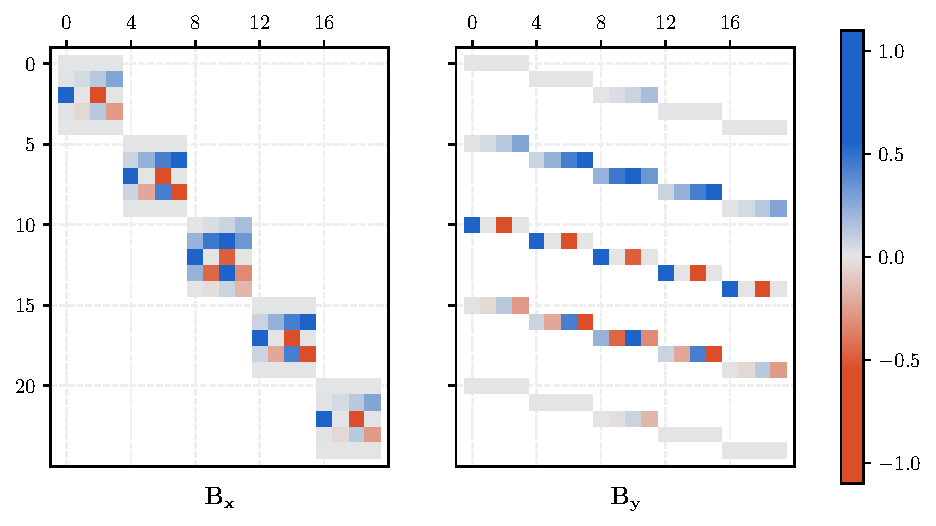
\includegraphics[width=\textwidth]{img/chapter4/new_method_beta.pdf}
        \caption{The non-zero entries from the matrices $\vb{B_x}$ and $\vb{B_y}$ from equation \eqref{equ:c4_new_method_beta_definition} are visualized. These were calculated on the problem from section \ref{sec:c4_new_method_ixaru} with a 5 by 5 internal grid and 4 basis functions per line. In practice, these matrices are much larger.}
        \label{fig:c4_new_method_beta}
    \end{center}
\end{figure}

Lastly we define the matrices which contain the values of the basis functions in each of the grid points. For this let us define $m$ as the total number of intersection points. Now, we define the $m \times n_x$ matrix $\vb{B_x}$ and the $m \times n_y$ matrix $\vb{B_y}$. Each row $r$ of these matrices correspond to an intersection $(x_i, y_j)$. Matrix $\vb{B_x}$ is mostly zero, except, on row $r$, for the values in columns from $o_x := \sum_{i' < i} K_{x_{i'}}$ to before $o_x + K_i$. Analogous, is $\vb{B_y}$ mostly zero on row $r$, except for the values in the columns from $o_y := \sum_{j' < j} K_{y_{j'}}$ to before $o_y + K_{y_j}$. These non-zero entries are now given as:
\begin{align}
    \left(\vb{B_x}\right)_{r, o_x + k} & =  \beta_{k}^{(x_i)}(y_j) \text{ for $k \in \{0, 1, \dots, K_{x_i} - 1\}$ }   \nonumber                               \\
    \text{and }
    \left(\vb{B_y}\right)_{r, o_y + k} & =  \beta_{k}^{(y_j)}(x_i) \text{ for $k \in \{0, 1, \dots, K_{y_i} - 1\}$.} \label{equ:c4_new_method_beta_definition}
\end{align}
To aid an intuitive understanding of the $\vb{B_x}$ and $\vb{B_y}$ matrices, figure \ref{fig:c4_new_method_beta} provides a schematic view of them, calculated from a small numerical example.


As promised, these definitions allow us to rewrite the system \eqref{equ:c4_new_method_pre_matrix_unified} with $m$ equations more compactly as:
$$
    \vb{B_x} \vb{\Lambda_x}\vb{c_x} + \vb{B_y} \vb{\Lambda_y}\vb{c_y} = E \vb{B_x} \vb{c_x} = E \vb{B_y} \vb{c_y}\text{.}
$$
This formulation is not yet reminiscent of any classical linear algebra problem. One of the unfamiliar parts of this expression is the fact that there are two vectors of unknowns, another unfamiliar part is that this are, in fact, two different problems.
\begin{equation}
    \begin{cases}
        \vb{B_x} \vb{\Lambda_x}\vb{c_x} + \vb{B_y} \vb{\Lambda_y}\vb{c_y} = E \vb{B_x} \vb{c_x} \\
        \vb{B_x} \vb{c_x} = \vb{B_y} \vb{c_y}
    \end{cases} \label{equ:c4_new_method_first_matrix_problem}
\end{equation}

There are a few strategies to further translate this problem into a form for which efficiently implemented and well-studied algorithms exist. Ideally, the solution would take the sparsity of the involved matrices into account.

\subsection{Solving the matrix approximation}

As a first strategy we researched how this problem can be directly transformed into a known type of problem.

\subsubsection{By direct transformation into an eigenvalue problem}

We tackle equation \eqref{equ:c4_new_method_first_matrix_problem} by rewriting it as
$$
    \begin{cases}
        \vb{B_x} \vb{\Lambda_x}\vb{c_x} + \vb{B_y} \vb{\Lambda_y}\vb{c_y} = E \vb{B_x} \vb{c_x} \\
        \vb{B_x} \vb{\Lambda_x}\vb{c_x} + \vb{B_y} \vb{\Lambda_y}\vb{c_y} = E \vb{B_y} \vb{c_y} \\
    \end{cases}\text{.}
$$
This system can be seen as the following generalized rectangular eigenvalue problem:
\begin{equation}\label{equ:c4_new_method_alternative_system}
    \begin{pmatrix}
        \vb{B_x} \vb{\Lambda_x} & \vb{B_y} \vb{\Lambda_y} \\
        \vb{B_x} \vb{\Lambda_x} & \vb{B_y} \vb{\Lambda_y}
    \end{pmatrix} \begin{pmatrix}
        \vb{c_x} \\ \vb{c_y}
    \end{pmatrix} = E \begin{pmatrix}
        \vb{B_x} & \vb{0} \\ \vb{0} & \vb{B_y}
    \end{pmatrix} \begin{pmatrix}
        \vb{c_x} \\ \vb{c_y}
    \end{pmatrix}\text{.}
\end{equation}

At first glance this may seem to enable us to solve the problem elegantly. But, there are a few issues apparent with this translation. One of the most visible problems is that we have translated this into a matrix problem which is twice as large in both rows and columns. On the other hand, one can argue, the matrices are clearly sparse. The matrices $\vb{B_x}$ and $\vb{B_y}$ are sparse indeed, but the problem is that there are few algorithms available that are able to solve a generalized rectangular eigenvalue problem, let alone a sparse one.

But a lack of sparse implementations, does not deter us from trying out some numerical experiments. In this first experiment we will have to fall back to algorithms working on dense matrices. Of course, the runtime will suffer, but from a numerical point of view the results will still be valuable.

Consider the Schrödinger equation with the harmonic oscillator potential:
$$
    -\nabla^2\psi(x, y) + \left(x^2 + y^2\right) \psi(x, y) = E \psi(x, y)
$$
on the domain $[-10, 10] \times [-10, 10]$ with homogeneous Dirichlet boundary conditions. We apply the described method on a grid with 30 lines in each direction and 15 basis functions per line. This yields $900\times 420$ matrices $\vb{B_x}$ and $\vb{B_y}$, and the rectangular problem from \eqref{equ:c4_new_method_alternative_system} has \numprint{1800} equations and \numprint{840} variables. As this eigenvalue problem is heavily overdetermined, we have to considered that solutions will only be accurate in a least squares sense. Much research is already dedicated to solving this kind of problem, as such we will, for now, use the first method from \cite{hua_svd_1991} to find solutions. Later on, we will explore the world of generalized rectangular eigenvalue problems.

If we write equation \eqref{equ:c4_new_method_alternative_system} symbolically as $\vb{A} \vb{c} = E \vb{D} \vb{c}$, and the truncated singular value decomposition of $\vb{D}$ as $\vb{D} = \vb{U_D} \vb{\Sigma_D} \vb{V_D^\adjointsign}$, then any solution of \eqref{equ:c4_new_method_alternative_system} will also be a solution of the generalized square eigenvalue problem
$$
    \vb{U_D^\adjointsign} \vb{A} \vb{V_D} \vb{v} = E \vb{\Sigma_D} \vb{v} \text{,}
$$
with $\vb{c} = \vb{V_D} \vb{v}$. Applying this method to the numeric problem yields 840 eigenvalues. Firstly, it is important to remark that the resulting values are elements of $\CC$. But, in this case, the imaginary part of all values lies between \numprint{-1.36e-14} and \numprint{1.36e-14}. So all values may be considered real. The lowest few values are given:
$$
    \underbrace{
        \numprint{-3.75e-14} \quad \dots \quad \numprint{5.59e-14}
    }_\text{196 values close to zero} \quad \numprint{2.00} \quad \numprint{3.46} \quad \numprint{3.46} \quad \numprint{4.00} \quad \numprint{4.00} \quad \dots
$$

This can be more compactly summarized when repeated values are indicated by a subscript:
$$
    \numprint{0.00}_{196} \quad \numprint{2.00} \quad \numprint{3.46}_2 \quad \numprint{4.00}_2 \quad \numprint{4.89}_2 \quad \numprint{6.00}_3 \quad \numprint{6.12}_2 \quad \dots \quad \numprint{7.73}_2 \quad \numprint{8.00}_4\quad \dots
$$

One immediately notices the many returned zero values. This does not have to be surprising, in fact, the matrix on the left-hand side of \eqref{equ:c4_new_method_alternative_system} may not be of full rank. But these zeros indicate another problem. Namely, that for these values it is not at all guaranteed that $\vb{B_x} \vb{c_x} = \vb{B_y} \vb{c_y}$.

Remember that the true eigenvalues of the harmonic oscillator are 2, 4, 4, 6, 6, 6, 8, 8, 8, 8, \dots. And, we notice that these true values can indeed be found in our solutions. But also many other values are present. Because the method from \cite{hua_svd_1991} for solving generalized rectangular eigenvalue problems may return more solutions than the original problems has, we still have to filter some out. One way to only end up with true eigenvalues is by substituting them back into the original problem \eqref{equ:c4_new_method_first_matrix_problem} and verifying the residuals of both equations:
$$
    r_1 = \left\| \vb{B_x} \vb{\Lambda_x} \vb{c_x} + \vb{B_y} \vb{\Lambda_y} \vb{c_y} - \frac{E}{2}\left(\vb{B_x}\vb{c_x} + \vb{B_y}\vb{c_y}\right) \right\| \text{ and } r_2=\left\| \vb{B_x} \vb{c_x} - \vb{B_y} \vb{c_y} \right\|\text{.}
$$

The found possible eigenvalue with the lowest residuals $r_1$ and $r_2$ are also true eigenvalues of the Schrödinger problem. When we sort all possibilities by their first residual $r_1$ we obtain the following table.

\begin{center}
    \begin{tabular}{r|rrrrr}
$E$ & \numprint{2.000000} & \numprint{4.000000} & \numprint{4.000000} & \numprint{6.000000} & \numprint{7.999998} \\\hline
$r_1$ & \numprint{1.5e-5} & \numprint{4.7e-4} & \numprint{4.7e-4} & \numprint{4.9e-4} & \numprint{5.0e-3} \\
$r_2$ & \numprint{1.2e-5} & \numprint{2.3e-4} & \numprint{2.3e-4} & \numprint{1.6e-4} & \numprint{1.2e-3}
\end{tabular}

\begin{tabular}{r|rrrrr}
$E$ & \numprint{7.999998} & \numprint{9.999997} & \numprint{9.999997} & \numprint{10.000006} & \numprint{8.000007} \\\hline
$r_1$ & \numprint{5.0e-3} & \numprint{6.6e-3} & \numprint{6.7e-3} & \numprint{1.0e-2} & \numprint{1.4e-2} \\
$r_2$ & \numprint{1.2e-3} & \numprint{1.3e-3} & \numprint{1.3e-3} & \numprint{2.1e-3} & \numprint{3.5e-3}
\end{tabular}

\begin{tabular}{r|rrrrr}
$E$ & \numprint{8.000007} & \numprint{13.999988} & \numprint{5.999974} & \numprint{5.999974} & \numprint{10.000151} \\\hline
$r_1$ & \numprint{1.4e-2} & \numprint{1.9e-2} & \numprint{3.8e-2} & \numprint{3.8e-2} & \numprint{4.8e-2} \\
$r_2$ & \numprint{3.5e-3} & \numprint{2.7e-3} & \numprint{1.3e-2} & \numprint{1.3e-2} & \numprint{9.6e-3}
\end{tabular}


\end{center}

Here, we see that when the first residual $r_1$ is low, the other is as well. Also, in the first few eigenvalues, only true solutions are present.

Upon studying this direct method to solve the system of equations \eqref{equ:c4_new_method_first_matrix_problem}, we have noticed some drawbacks. Firstly, the proposed system \eqref{equ:c4_new_method_alternative_system} is, in a certain sense, twice as large as the discrete problem we started from. Eigenvalue algorithms are at least cubic in complexity. So, this doubling in size implies an eightfold runtime penalty Secondly, and numerically interesting, we obtain many more `solutions' than the ones we are looking for. Each generalized eigenvalue, with its eigenvector, has to be computed and checked against the residuals. Many eigenvalues will be thrown away.

\subsubsection{By restriction to a null space}

One improvement we can make to the runtime is by not solving a system that is twice as large, but by solving two, smaller, systems. Furthermore, instead of ending up with to many eigenvalues and trying to filter out the wrong ones, we have devised a way to a priori already limit the number of solutions. The idea here is that, before solving an eigenvalue problem, we solve the second equation of \eqref{equ:c4_new_method_first_matrix_problem} and only take those solutions into account.

The first equation resembles a generalized rectangular eigenvalue problem, the second is a classical linear system. Let us only consider $n_x + n_y$ dimensional vectors $\vb{c} = \transpose{\begin{pmatrix}\transpose{\vb{c_x}} & \transpose{\vb{c_y}} \end{pmatrix}}$ which solve
$$
    \begin{pmatrix}\vb{B_x} & -\vb{B_y} \end{pmatrix} \vb{c} = \vb{0}\text{.}
$$
This allows us to unify $\vb{c_x}$ and $\vb{c_y}$, while ensuring $\vb{B_x} \vb{c_x} = \vb{B_y} \vb{c_y}$ is satisfied. To expand on this idea, we will write $\vb{c}$ to be an element of the right kernel of  $\begin{pmatrix}\vb{B_x} & -\vb{B_y} \end{pmatrix}$. For this define $\vb{Z}$ to be the $(n_x + n_y) \times z$-dimensional basis of this right kernel:
\begin{equation}\label{equ:c4_null_space_kernel}
    \begin{pmatrix}\vb{B_x} & -\vb{B_y} \end{pmatrix} \vb{Z} = \vb{0}\text{.}
\end{equation}

Computing this kernel numerically is definitely not trivial. For rectangular matrices, there are a few much used methods to compute the kernel. In the next few paragraphs we will explore these methods and consider how well they are suited for our problem. For ease of notation we will be solving the rectangular system $\vb{A} \vb{Z} = \vb{0}$ with $\vb{A}$ a (sparse) $n\times m$ matrix and $\vb{Z}$ a yet unknown basis $\vb{m} \times \vb{k}$ for the right null space of $\vb{A}$.

One of the first methods one finds browsing the literature ({\color{red}To do: a nice reference to a textbook}), is by using a QR-decomposition with pivoting. For this we decompose the matrix as $\transpose{\vb{A}}\vb{E} = \vb{Q} \vb{R}$, with $\vb{E}$ a permutation matrix, $\vb{Q}$ a square orthogonal matrix and $\vb{R}$ a rectangular upper triangular matrix, with the elements on its diagonal sorted (descending in absolute value). To find the kernel we now consider for which vectors $\vb{Z}$ the expression $\vb{A} \vb{z} = \vb{E}\transpose{\vb{R}}\transpose{\vb{Q}}$ becomes zero. Notice that this only happens when $\vb{z}$ is one of the columns of $\vb{Q}$, corresponding to a diagonal item in $\vb{R}$ that does not exist or is (close to) zero. So an orthogonal basis of the null space of $\vb{A}$ can simply be found in a selection of columns of $\vb{Q}$ in the QR-decomposition of $\transpose{\vb{A}}$. For dense matrices this procedure works very well. We can quite easily compute the full kernel with built-in QR routines. Upon selecting which columns to include, the diagonal elements of $\vb{R}$ can even be used to respect a prespecified tolerance. But for sparse matrices, the story is quite different. There are many well-tested routines to compute sparse QR decompositions (SPQR, Eigen's QR, and scipy's). Yet, we have tested this algorithm with many different solvers, without success. Some implementations do not contain a rank revealing QR decomposition, and as such are unable to compute the full kernel. With other implementations were sometimes able to compute the kernel. But this computation was each time very sensitive to the tolerances for when pivoting should happen. Even worse, the perfect 'tolerance' was different for each test problem, or even the same problem with different parameters.

Note that numerically, it is impossible to consider the exact kernel. {\color{red} To do: the numerical treatment of the computation of this kernel.}

The vector $\vb{c}$ can now be written as a certain linear combination of columns of $\vb{Z}$:
$$
    \vb{c} = \begin{pmatrix}\vb{c_x} \\ \vb{c_y} \end{pmatrix} = \begin{pmatrix} \vb{Z_x} \\ \vb{Z_y} \end{pmatrix}  \vb{u} = \vb{Z} \vb{u} \text{.}
$$
Another benefit of considering $\vb{Z}\vb{u}$, besides only considering solutions of $\vb{B_x} \vb{c_x} = \vb{B_y} \vb{c_y}$, is that we unified the two vectors of unknowns $\vb{c_x}$ and $\vb{c_y}$ into one (much) smaller vector $\vb{u}$. This simplifies the two problems of equation \eqref{equ:c4_new_method_first_matrix_problem} into
$$
    \begin{pmatrix}
        \vb{B_x}\vb{\Lambda_x} & \vb{B_y}\vb{\Lambda_x}
    \end{pmatrix} \vb{Z} \vb{u} = E \vb{B_x} \vb{Z_x} \vb{u} = E \vb{B_y} \vb{Z_y} \vb{u} \text{.}
$$
For the right-hand side, by construction $\vb{B_x} \vb{Z_x} = \vb{B_y} \vb{Z_y}$. Now, this problem has become a generalized rectangular eigenvalue problem.


\subsubsection{Finding solutions of generalized rectangular eigenvalue problems}

{\color{red} To do: A small word about this kind of problem.}

\subsection{Computing eigenfunctions}

\subsection{Numerical experiments}

\subsubsection{Ixaru's potential}\label{sec:c4_new_method_ixaru}

\subsection{Comparing run time with the finite difference method}\label{sec:c4_nm_vs_fd}

\section{Some ideas for a utopian method}\label{c4:sec_utopy}


\stopchapter
